\documentclass[ProjectRequirements.tex]{subfiles}
\begin{document}

\bigskip

\section{\textsc{\Large Overall Description}}
	\begin{figure}[H]
		\centering
		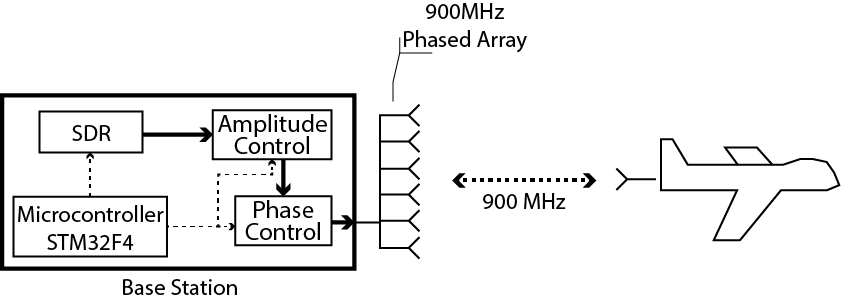
\includegraphics[]{HardwareBlockDiagram.png}
		\caption{Hardware Block Diagram \label{fig:HardwareBlockDiagram}}
		\clearpage
		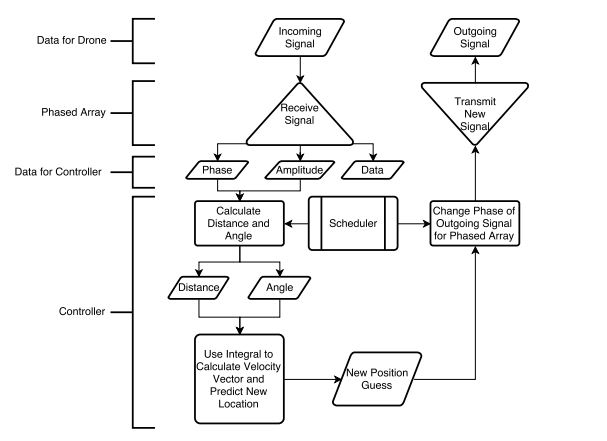
\includegraphics[]{SoftwareBlockDiagram.png}
		\caption{Tracking Block Diagram \label{fig:SoftwareBlockDiagram}}
	\end{figure}
	\subsection{Product Perspective}
	
		\subsubsection{System Interfaces}
			
		\subsubsection{User Interfaces}
			The system must have a UART port through which the user can establish a serial connection. The user should be able to modify various settings through this port. This port must conform to the following requirements:
			\begin{enumerate}
				\item When a connection is established, the interface must send a list of instructions and changeable parameters over the UART.
				\item The interface must be straightforward enough that a technical user can use the instructions to configure the settings within 20 minutes.
				\item There must be clear documentation about each setting describing (1) what it does, (2) why it's valuable, and (3) how to use it.
			\end{enumerate}	
			
		\subsubsection{Hardware Interfaces}
			\begin{itemize}\itemsep1pt
				\item \textbf{STM32F4} -- 
				\item \textbf{Xeta SDR} -- 
				\item \textbf{Phased Array} -- 
			\end{itemize}
			
		\subsubsection{Software Interfaces}
			\begin{enumerate}\itemsep1pt
				\item 
			\end{enumerate}
			
		\subsubsection{Communications Interfaces}
			\begin{itemize}\itemsep1pt
				\item 
			\end{itemize}
			
		\subsubsection{Memory}
			\begin{itemize}\itemsep1pt
				\item 
			\end{itemize}
		
		\subsubsection{Operations}
			\begin{itemize}\itemsep1pt
				\item 
			\end{itemize}
		
	\subsection{Product Functions}
	
		\subsubsection{High Priorities}
			\begin{enumerate}
				\item \textbf{Distance} -- The 900MHz phased array must be able to establish a connection with a drone in motion up to 20 miles away. !!! WHAT DOES IT MEAN TO ESTABLISH A CONNECTION? !!!
				\item \textbf{Power} -- The 900MHz phased array must never exceed the FCC maximum power specifications, which is 4 watts.
				\item \textbf{Command Transmission Rate} -- The 900MHz phased array must be able to transmit telemetry at 10Hz.
				\item \textbf{Cost} -- The project should cost no more than \$10,000 to produce the prototype
							
			\end{enumerate}
		
		\subsubsection{Medium Priorities}
			\begin{enumerate}
				\item \textbf{Communications} -- The communications should be radio agnostic. !!! COME BACK HERE AND MAKE THIS MORE DETAILED !!!
				\item \textbf{Stacked Antennas} -- The 2.4GHz phased array must be able to establish a connection with a drone in motion up to 5 miles away.
			\end{enumerate}
		
		\subsubsection{Low Priorities}
			\begin{enumerate}
				\item \textbf{Multiplexing} -- The phased arrays should be able to simultaneously communicate with up to 4 drones at once while maintaining a lock.
				\item \textbf{Video} -- The 
			\end{enumerate}
		
	\subsection{User Characteristics}
	
	\subsection{Design Constraints}
	
	\subsection{Assumptions and Dependencies}
	
\end{document}
